\subsection{Background}
SYN Flooding Attack is a denial-of-service (DoS) attack which means that its goal is to make its victim unavailable for legitimate traffic by ''flooding'' its response resources. This attack causes all resources to be used up so that the victim is unable to properly respond to the handshake for legitimate clients. As Fig. 1 shows the Attacker uses Bots or an attack script to send many SYN Packets/Messages to the Victim using a spoofed address. When the Victim gets these SYN Messages, the Victim replies back with its SYN-ACK to approve the connection requests but the Attacker does not reply to them causing the SYN-ACK to hang. It takes resources to send and keep the SYN-ACKs, so the Victim eventually runs out of resources causing the Victim to fail. 

\subsection{Flood Attack Demonstration Setup}
To demonstrate this attack, I first set up a virtual network named ''tcpattack'' on the subnet 10.2.5.0/24 using a Virtual Machine (VM) running an Ubuntu 24.04 image. On the virtual network, I set up three different containers: Victim (10.2.5.5), Attacker (Host) and Client (10.2.5.6). 
\begin{figure}[h]
    \centering
    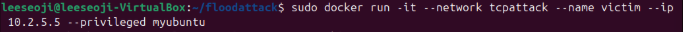
\includegraphics[width=\columnwidth]{images/flood attack/docker_victim.png}
    \caption{Creating Victim Container}
    \label{fig:docker_victim}
\end{figure}
\begin{figure}[h]
    \centering
    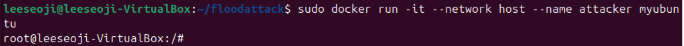
\includegraphics[width=\columnwidth]{images/flood attack/docker_attacker.png}
    \caption{Creating Attacker Container}
    \label{fig:docker_attacker}
\end{figure}
\begin{figure}[h]
    \centering
    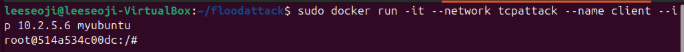
\includegraphics[width=\columnwidth]{images/flood attack/docker_client.png}
    \caption{Creating Client Container}
    \label{fig:docker_client}
\end{figure}  

The Victim container would help to demonstrate the incoming number of Packets, the Attacker would run the attacking script and the Client container would help to simulate legitimate user traffic and demonstrate the denial of service effect on the Victim during the attack.

With the three containers created, I first set up the Victim container. I made it a simple Python webserver using the ''Python 3 -m http.server 8080'' command. This command sets up a simple http server running on the port 8080. With this server up, using the ''Curl 10.2.5.5:8080'' command on the Client container, it should show the html of the Python server as seen in Fig.~\ref{fig:good_curl_response}.

\begin{figure}[h]
    \centering
    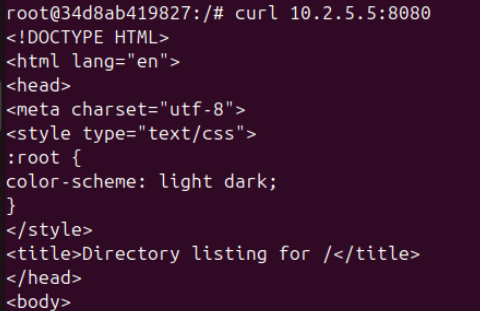
\includegraphics[width=0.8\columnwidth]{images/flood attack/good_curl_response.png}
    \caption{Successful curl of Victim Server }
    \label{fig:good_curl_response}
\end{figure} 


After seeing that the Victim and Client is working, I worked on the Attacker container. For the Attacker, I wrote a flood attack script named ``syn\_flood.py'' using the Scapy library as seen in Fig.~\ref{fig:syn_flood_script}.
 
\begin{figure}[h]
    \centering
    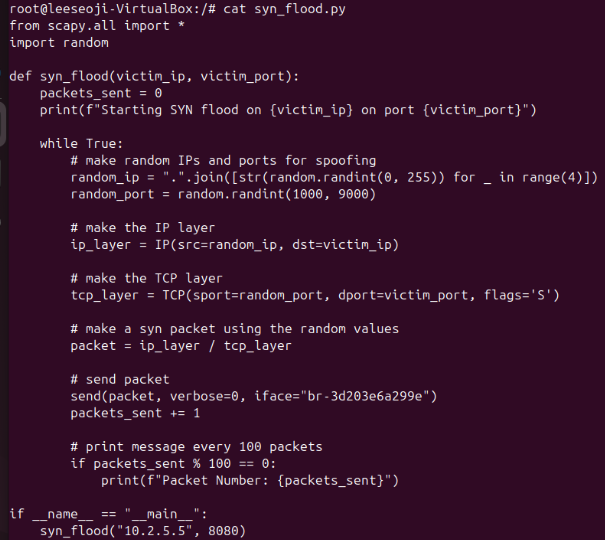
\includegraphics[width=0.8\columnwidth]{images/flood attack/flood_attack_script.png}
    \caption{SYN Flood attack script written using Scapy library}
    \label{fig:syn_flood_script}
\end{figure}  

The script uses a while loop where in each loop, it creates a random/spoofed IP address and Port number and uses that to generate a IP layer and TCP layer. Using the two layers, it then creates a TCP packet and sends that to the victim on port 8080. Because it uses a while loop, the script will generate and send packets until the script is manually shut off. 

\subsection{Flood Attack Demonstration}
To demonstrate the attack, I first ran the Python server on the Victim container, then started the flood attack script as seen in Fig.~\ref{fig:flood_attack_script_running}.
\begin{figure}[h]
    \centering
    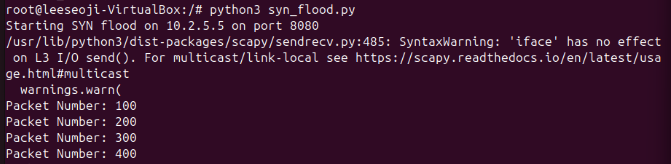
\includegraphics[width=0.8\columnwidth]{images/flood attack/flood_attack_script_running.png}
    \caption{Flood Attack Script Running}
    \label{fig:flood_attack_script_running}
\end{figure} 

As the attack was being carried out, I would check on the Client Container running the Curl command to see the connection would still work. Within the first few hundred packets sent, the connection would still work, however after reaching around the thousand mark, the Curl command would significantly slow down in response, and end up resulting in the timeout error which successfully demonstrated the denial of service effect as seen in Fig.~\ref{fig:bad_curl_response}.

\begin{figure}[h]
    \centering
    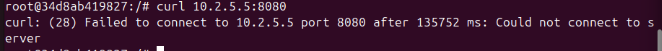
\includegraphics[width=\columnwidth]{images/flood attack/bad_curl_response.png}
    \caption{Connection Time Out Message}
    \label{fig:bad_curl_response}
\end{figure}

The number of packets being sent to the Victim can also be visualized by using Wireshark as in Fig.~\ref{fig:wireshark_home} and Fig.~\ref{fig:wireshark_packet_number}.

\begin{figure}[h]
    \centering
    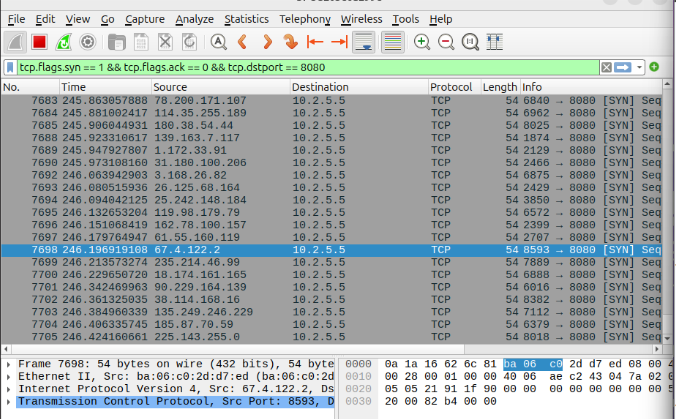
\includegraphics[width=0.7\columnwidth]{images/flood attack/wireshark_home.png}
    \caption{Visualization of Packets incoming in Wireshark}
    \label{fig:wireshark_home}
\end{figure}

\begin{figure}[h]
    \centering
    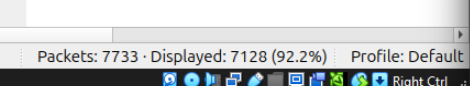
\includegraphics[width=\columnwidth]{images/flood attack/wireshark_packet_number.png}
    \caption{The number of Packets sent to Victim}
    \label{fig:wireshark_packet_number}
\end{figure}


\subsection{Flood Attack Mitigation Techniques}
The SYN Flooding attack has mitigation techniques that can be applied to improve security. The mitigation techniques that I tried were: Enabling SYN Cookies, Increasing the backlog Queue and Recycling old half open TCP connections. 

\begin{enumerate}
    \item \textbf{Enable SYN Cookies} \\
    The first technique was to enable SYN Cookies. Enabling SYN cookies helps to eliminate the need for the server to use resources for half-open connections. It allows for the use of cryptographic cookies for the SYN-ACK response and only uses resources for connections that reach the last ACK stage. SYN Cookies helps to solve the resource issues which the flood attack exploits, so it helps to mitigate the attack. To enable SYN Cookies, the following command was used:
    \begin{figure}[h]
        \centering
        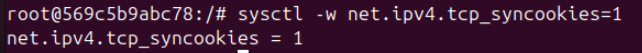
\includegraphics[width=\columnwidth]{images/flood attack/syn_cookies.png}
        \caption{Enabling SYN Cookies}
        \label{fig:syn_cookie}
    \end{figure}
    
    With SYN Cookies enabled, the Client was able to 
    successfully connect to the Victim server using curl even while the flood attack script was actively running, demonstrating complete mitigation of the attack.

    \item \textbf{Increase SYN Backlog Queue} \\
   The second technique was to increase the SYN backlog queue. This increases the amount of half-open connections that the server can handle so it increases the number of connections that the server can handle before failing. To increase the backlog queue size, the following command was used:
    \begin{figure}[h]
        \centering
        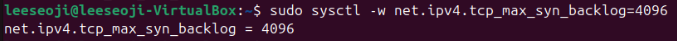
\includegraphics[width=\columnwidth]{images/flood attack/increase_backlog_queue.png}
        \caption{Increasing Backlog Queue}
        \label{fig:Increasing Backlog Queue}
    \end{figure}
    
    While this technique allowed the server to remain 
    available for a longer period of time, it did not 
    completely stop the attack as the queue would eventually fill up when the flood script ran for extended time.

    \item \textbf{Recycle Old Half-Open TCP Connections} \\
    The last technique I tried was to recycle old half-open TCP connections. This overwrites the old half-open connections when the backlog is full rather than using more resources. To enable connection recycling, the following command was 
    used:
    \begin{figure}[h]
        \centering
        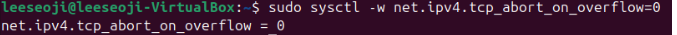
\includegraphics[width=\columnwidth]{images/flood attack/recycle_old_connections.png}
        \caption{Recycle Old Half-Open TCP Connections}
        \label{fig:Recycle Old Half-Open TCP Connections}
    \end{figure}
    
    With this technique enabled, the Client was able to 
    connect to the Victim server during the attack, however the connection was noticeably slower than normal due to the server still being heavy burdened from processing the flood of incoming packets.
\end{enumerate}

Out of the three mitigation techniques, enabling SYN cookies was the most effective at mitigating the effects of the attack. In a real-life environment, using all three techniques would result in the best results. 
